\documentclass{beamer}

\mode<presentation> {

%\usetheme{default}
%\usetheme{AnnArbor}
%\usetheme{Antibes}
%\usetheme{Bergen}
%\usetheme{Berkeley}
%\usetheme{Berlin}
%\usetheme{Boadilla}
%\usetheme{CambridgeUS}
%\usetheme{Copenhagen}
%\usetheme{Darmstadt}
%\usetheme{Dresden}
%\usetheme{Frankfurt}
%\usetheme{Goettingen}
%\usetheme{Hannover}
%\usetheme{Ilmenau}
%\usetheme{JuanLesPins}
%\usetheme{Luebeck}
\usetheme{Madrid}
%\usetheme{Malmoe}
%\usetheme{Marburg}
%\usetheme{Montpellier}
%\usetheme{PaloAlto}
%\usetheme{Pittsburgh}
%\usetheme{Rochester}
%\usetheme{Singapore}
%\usetheme{Szeged}
%\usetheme{Warsaw}


%\usecolortheme{albatross}
%\usecolortheme{beaver}
%\usecolortheme{beetle}
%\usecolortheme{crane}
%\usecolortheme{dolphin}
%\usecolortheme{dove}
%\usecolortheme{fly}
%\usecolortheme{lily}
%\usecolortheme{orchid}
%\usecolortheme{rose}
%\usecolortheme{seagull}
%\usecolortheme{seahorse}
%\usecolortheme{whale}
%\usecolortheme{wolverine}

%\setbeamertemplate{footline} % To remove the footer line in all slides uncomment this line
%\setbeamertemplate{footline}[page number] % To replace the footer line in all slides with a simple slide count uncomment this line

%\setbeamertemplate{navigation symbols}{} % To remove the navigation symbols from the bottom of all slides uncomment this line
}

\usepackage{graphicx} % Allows including images
\usepackage{booktabs} % Allows the use of \toprule, \midrule and \bottomrule in tables
\usepackage{amsfonts}
\usepackage{mathrsfs}
\usepackage{amsmath,amssymb,graphicx}

\newcommand{\verbatimfont}[1]{\renewcommand{\verbatim@font}{\ttfamily#1}} % small verbatim

%----------------------------------------------------------------------------------------
%	TITLE PAGE
%----------------------------------------------------------------------------------------

\title["1.4"]{1.4: Stationary Models and the Autocorrelation Function} 

\author{Taylor} 
\institute[UVA] 
{
University of Virginia \\
\medskip
\textit{} 
}
\date{} 

\begin{document}
%----------------------------------------------------------------------------------------

\begin{frame}
\titlepage 
\end{frame}
%----------------------------------------------------------------------------------------

\begin{frame}
\frametitle{Definition}

\begin{block}{defn}
$\{X_t\}$ is {\bf strictly stationary} if for any $h$, and any selection of $k$ time points ($t_1, \ldots, t_k$):
\[
F_{X_{t_1 + h}, \ldots, X_{t_k +h}}(a_1, \ldots, a_k) = F_{X_{t_1}, \ldots, X_{t_k }}(a_1, \ldots, a_k),
\]
for any $a_1, \ldots, a_k$.
\end{block}

Intuitively this means that the distribution of a bunch of time points does NOT depend on where they are in time, only on how they are spaced apart from one another.
\newline

More often we will be concerned with \emph{weak} stationarity.

\end{frame}

%----------------------------------------------------------------------------------------

\begin{frame}
\frametitle{Definition}

Let $\{X_t\}$ be a time series with $E[X_t] < \infty$ for each $t$.

\begin{block}{mean function}
The {\bf mean function} is defined as
\[
\mu_X(t) = E[X_t]
\]
\end{block}

\begin{block}{covariance function}
The {\bf covariance function} is defined on pairs of integral time points $r,s$ as 
\begin{align*}
\gamma_{X}(r,s) &= \text{Cov}(X_r, X_s) \\
&= E[(X_r - E[X_r])(X_s-E[X_s])] \\
&= E[X_rX_s] - E[X_r]E[X_s].
\end{align*}
\end{block}

\end{frame}

%----------------------------------------------------------------------------------------

\begin{frame}
\frametitle{Definition}

\begin{block}{weak stationarity}
$\{X_t\}$ is {\bf weakly stationary} if 
\begin{enumerate}
\item $\mu_X(t)$ is constant or free of $t$
\item $\gamma_X(t,t+h)$ is independent or free of $t$ for each $h$ 
\end{enumerate}
\end{block}
Intuitively: mean doesn't change, and covariances only depend on the lags.
\newline

From now on, when we say ``stationary," we mean this type.

\end{frame}

%----------------------------------------------------------------------------------------

\begin{frame}
\frametitle{Definition}

\begin{block}{The ACVF}
The {\bf autocovariance function} for $\{X_t\}$ is defined as
\[
\gamma_X(h) = \text{Cov}(X_{t+h},X_t).
\]
\end{block}
``Auto" means ``self"
\newline

\begin{block}{The ACF}
The {\bf autocorrelation function} for $\{X_t\}$ is defined as
\[
\rho_X(h) = \text{Cor}(X_{t+h},X_t) = \frac{ \text{Cov}(X_{t+h},X_t) }{ \sqrt{\text{Var}(X_t)\text{Var}(X_{t+h})}} = \frac{\gamma_X(h)}{\gamma_X(0)}.
\]
\end{block}
Because we are only defining this function for stationary series
\end{frame}

%----------------------------------------------------------------------------------------

\begin{frame}
\frametitle{Properties}

\begin{block}{Property 1}
The covariance operator is {\bf bilinear}: 
\begin{itemize}
\item $\text{Cov}(aX,Y) = a\text{Cov}(X,Y)$
\item $\text{Cov}(X,aY) = a\text{Cov}(X,Y)$
\item $\text{Cov}(X+Z,Y) = \text{Cov}(X,Y) + \text{Cov}(Z,Y)$
\item $\text{Cov}(X,Y+Z) = \text{Cov}(X,Y) + \text{Cov}(X,Z)$
\end{itemize}
\end{block}
``bi" means ``two" or ``both" (linear in both arguments)
\newline

\begin{block}{Property 2}
Independence implies (is stronger than) $0$ correlation/covariance
\begin{align*}
\gamma_X(h) = E[X_tX_{t+h}] - E[X_t]E[X_{t+h}] =  E[X_t]E[X_{t+h}] - E[X_t]E[X_{t+h}] = 0 
\end{align*}
\end{block}

We use these properties a lot when we look at autocovariance functions for different models.
\end{frame}

%----------------------------------------------------------------------------------------

\begin{frame}
\frametitle{Example 1: IID Noise}

Let $\{X_t\}$ be IID noise with $E[X_t] = 0$ and $\operatorname{Var}(X_t) = E[X_t^2] = \sigma^2 < \infty$. Then:

\[ 
\gamma_X(h) = E[X_{t+h}X_t] = 
  \begin{cases} 
      \sigma^2 & h = 0 \\
      0 & h \neq 0 
   \end{cases}
\]

\begin{itemize}
\item This is stationary.
\item We are not saying what the distribution is!
\item From now on we write $X_t \overset{iid}{\sim} \text{IID}(0, \sigma^2)$
\end{itemize}

\end{frame}

%----------------------------------------------------------------------------------------

\begin{frame}
\frametitle{Example 2: White Noise}

Let $\{X_t\}$ be uncorrelated but not necessarily independent with $E[X_t] = 0$ and $\operatorname{Var}(X_t) = E[X_t^2] = \sigma^2 < \infty$. Then:

\[ 
\gamma_X(h) = E[X_{t+h}X_t] = 
  \begin{cases} 
      \sigma^2 & h = 0 \\
      0 & h \neq 0 
   \end{cases}
\]

\begin{itemize}
\item This is stationary.
\item We are not saying what the distribution is!
\item From now on we write $X_t \overset{iid}{\sim} \text{WN}(0, \sigma^2)$
\item All IID Noise is White Noise, but not all White Noise is IID Noise.
\end{itemize}

\end{frame}


%----------------------------------------------------------------------------------------

\begin{frame}
\frametitle{Example 3: Random Walk}

Let $\{X_t\}$ be uncorrelated but not necessarily independent with $E[X_t] = 0$ and $\operatorname{Var}(X_t) = E[X_t^2] = \sigma^2 < \infty$. Define the random walk as $S_t = \sum_{i=1}^t X_i$. Then:

\begin{align*}
\gamma_X(t+h,t) &= E[S_{t+h}S_t] \\
&= E\left[\left\{\sum_{i=1}^{t+h} X_i\right\} \left\{ \sum_{i=1}^t X_i \right\}\right] \\
&=  E\left[\left\{\sum_{i=1}^{t} X_i \right\} \left\{\sum_{i=1}^t X_i \right\}\right] \\
&= \sum_{i=1}^t E[X_i^2] \\
&=  t \sigma^2.
\end{align*}

% \begin{itemize}
% \item This is not stationary!
% \item We are not saying what the distribution is!
% \item From now on we write $X_t \overset{iid}{\sim} \text{WN}(0, \sigma^2)$
% \item All IID Noise is White Noise, but not all White Noise is IID Noise.
% \end{itemize}

\end{frame}


%----------------------------------------------------------------------------------------

\begin{frame}
\frametitle{Example 3: Random Walk}

Let $\{X_t\}$ be uncorrelated but not necessarily independent with $E[X_t] = 0$ and $\operatorname{Var}(X_t) = E[X_t^2] = \sigma^2 < \infty$. Define the random walk as $S_t = \sum_{i=1}^t X_i$. Then:

\[
\gamma_X(h) =  t \sigma^2.
\]

\begin{itemize}
\item This is NOT stationary.
\item We are not saying what the distribution is!
\item But $E[S_t] = E[\sum_{i=1}^t X_t] = \sum_{i=1}^t E[X_t] = 0$ by linearity.
\item no ``pattern" but variance increasing with horizon
\end{itemize}

\end{frame}

%----------------------------------------------------------------------------------------

\begin{frame}
\frametitle{Example 4: First-Order Moving Average MA(1) }

Let $\{Z_t\} \sim \text{WN}(0, \sigma^2)$. Define $\{X_t\}$ as
\[
X_t = Z_t + \theta Z_{t-1}
\]
with $t \in \mathbb{Z}$, and $\theta \in \mathbb{R}$. 
\newline

$E[X_t] = 0$ for all $t$ by linearity, and 
\begin{align*}
\gamma_X(h) &= E[X_{t+h}X_t] \\
&= E[(Z_{t+h} + \theta Z_{t+h-1})(Z_t + \theta Z_{t-1})]  \\
&= E[Z_{t+h}Z_t] + \theta E[Z_{t+h} Z_{t-1}] + \theta E[Z_{t+h-1}Z_t] + \theta^2E[Z_{t+h-1}Z_{t-1}]  \\
&= (1 + \theta^2) \gamma_Z(h) + \theta \gamma_Z(h+1) + \theta \gamma_Z(h-1)   \\
&= \begin{cases} 
      \sigma^2(1 + \theta^2) & h = 0 \\
      \sigma^2\theta & h = \pm 1 \\
      0 & |h| > 1
   \end{cases}
\end{align*}
\end{frame}

%----------------------------------------------------------------------------------------

\begin{frame}
\frametitle{Example 4: First-Order Moving Average MA(1) }

$E[X_t] = 0$ for all $t$ by linearity, and 
\begin{align*}
\rho_X(h) &= \frac{\gamma_X(h)}{\gamma_X(0)} \\
&= \begin{cases} 
      1 \\
      \theta/(1+\theta^2) & h = \pm 1 \\
      0 & |h| > 1
   \end{cases}
\end{align*}

\begin{itemize}
\item This is stationary
\end{itemize}

\end{frame}


%----------------------------------------------------------------------------------------

\begin{frame}
\frametitle{Example 5: First-Order Autoregression AR(1) }

Let $\{Z_t\} \sim \text{WN}(0, \sigma^2)$. Also, assume $-1 < \phi < 1$, and $E[Z_tX_s] = 0$ for $s < t$. Define $\{X_t\}$ as
\[
X_t = \phi X_{t-1} + Z_t \tag{*}
\]
with $t \in \mathbb{Z}$. 
\newline

\begin{enumerate}
\item $E[X_t] = \phi E[X_{t-1}]$ for all $t$, by linearity. 
\item And if $h > 0$
  \begin{align*}
    \gamma_X(h) &= E[X_{t+h}X_t] \\
    &= E[(\phi X_{t+h-1} + Z_{t+h})(X_t + Z_t)] \\
    &= \phi \gamma_X(h-1) 
  \end{align*}
\item $\gamma_X(0) = E[(\phi X_{t-1} + Z_t)^2] = \phi^2\gamma_X(0) + \sigma^2 \iff \gamma_X(0) = \frac{\sigma^2}{1-\phi^2 }$
\end{enumerate}



\end{frame}

%----------------------------------------------------------------------------------------

\begin{frame}
\frametitle{Example 5: First-Order Autoregression AR(1) }

Let $\{Z_t\} \sim \text{WN}(0, \sigma^2)$. Also, assume $-1 < \phi < 1$, and $E[Z_tX_s] = 0$ for $s < t$. Define $\{X_t\}$ as
\[
X_t = \phi X_{t-1} + Z_t \tag{*}
\]
with $t \in \mathbb{Z}$. 

\begin{enumerate}
\item If one has mean $0$, they all do, so we assume they all have mean $0$. 
\item Clearly $\gamma_X$ is symmetric, i.e. $\gamma_X(h) = \gamma_X(-h)$
\end{enumerate}

\begin{block}{AR(1) stationarity}
Under these assumptions, $\{X_t\}$ is stationary with $\mu_X(t) = 0$, $\gamma_X(h) = \phi^{|h|}\frac{\sigma^2}{(1-\phi^2)}$ and $\rho_X(h) = \phi^{|h|}$.
\end{block}

\end{frame}

%----------------------------------------------------------------------------------------

\begin{frame}
\frametitle{The Sample ACVF and ACF}

We never have the true/population autocovariance or autocorrelation function. So far we are just theorizing about made up models.
\newline

Enter the {\bf sample autocovariance and autocorrelation functions}. They estimate $\gamma_X$ and $\rho_X$.
\newline

\end{frame}

%----------------------------------------------------------------------------------------

\begin{frame}
\frametitle{The Sample ACVF and ACF}

The {\bf sample mean} of the data $x_1, \ldots, x_n$ is $\bar{x} = \frac{1}{n}\sum_{t=1}^n x_t.$

\begin{block}{The sample autocovariance function}
The {\bf sample autocovariance function} for the data $x_1, \ldots, x_n$ is
\[
\hat{\gamma}(h) = \frac{1}{n}\sum_{i=1}^{n-|h|}(x_{t+|h|}-\bar{x})(x_t - \bar{x}), \hspace{10mm} -n < h < n.
\]
\end{block}

\begin{block}{The sample autocorrelation function}
The {\bf sample autocorrelation function} for the data $x_1, \ldots, x_n$ is
\[
\hat{\rho}(h) = \frac{\hat{\gamma}(h)}{\hat{\gamma}(0)}, \hspace{10mm} -n < h < n.
\]
\end{block}

\end{frame}


%----------------------------------------------------------------------------------------

\begin{frame}
\frametitle{Test Yourself 1}

What model is appropriate for the following data?

\begin{center}
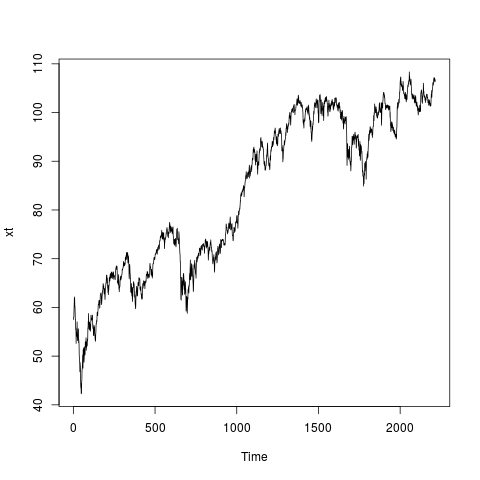
\includegraphics[width=100mm]{/home/taylor/UVa/all_teaching/4170_slides/1/1.4/pics/Rplot}
\end{center}

\end{frame}

%----------------------------------------------------------------------------------------

\begin{frame}
\frametitle{Test Yourself 1}

What about if we look at the sample autocorrelation?

\begin{center}
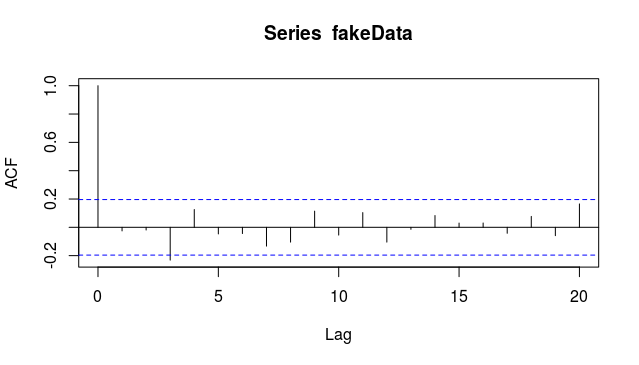
\includegraphics[width=100mm]{/home/taylor/UVa/all_teaching/4170_slides/1/1.4/pics/Rplot01}
\end{center}

The bounds are $95$\% confidence intervals, which means we should expect to see about $(100-95)$\% of the data to be accidentally outside this range.

\end{frame}

%----------------------------------------------------------------------------------------

\begin{frame}[fragile]
\frametitle{Test Yourself 1}

Answer: it was IID Gaussian Noise.
\begin{verbatim}
fakeData <- rnorm(n=100,mean = 0, sd = 2)
plot(fakeData, type = "b")
acf(fakeData, type = "correlation")
\end{verbatim}

\end{frame}


%----------------------------------------------------------------------------------------

\begin{frame}
\frametitle{Test Yourself 2}

Round 2: 

\begin{center}
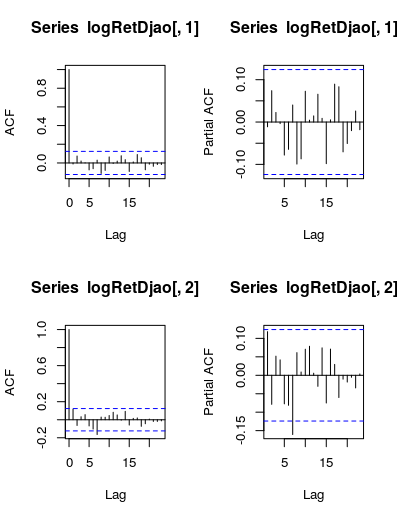
\includegraphics[width=100mm]{/home/taylor/UVa/all_teaching/4170_slides/1/1.4/pics/Rplot02}
\end{center}

\end{frame}

%----------------------------------------------------------------------------------------

\begin{frame}
\frametitle{Test Yourself 2}

Looking at the sample autocorrelation?

\begin{center}
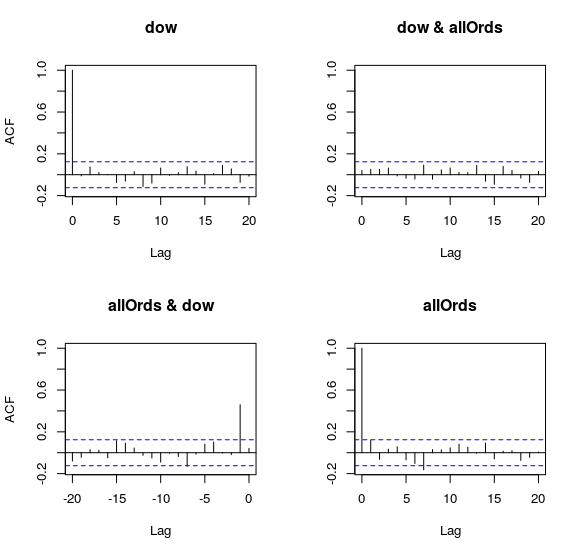
\includegraphics[width=100mm]{/home/taylor/UVa/all_teaching/4170_slides/1/1.4/pics/Rplot03}
\end{center}


\end{frame}


%----------------------------------------------------------------------------------------

\begin{frame}[fragile]
\frametitle{Test Yourself 2}

Answer: it was AR(1) with Gaussian Noise.
\begin{verbatim}
arima.sim(list(ar=c(.9)), n = 200)
plot(fakeData2, type = "b")
acf(fakeData2, type = "correlation")
\end{verbatim}

\end{frame}

%----------------------------------------------------------------------------------------

\begin{frame}[fragile]
\frametitle{Test Yourself 3}

Last one: 

\begin{center}
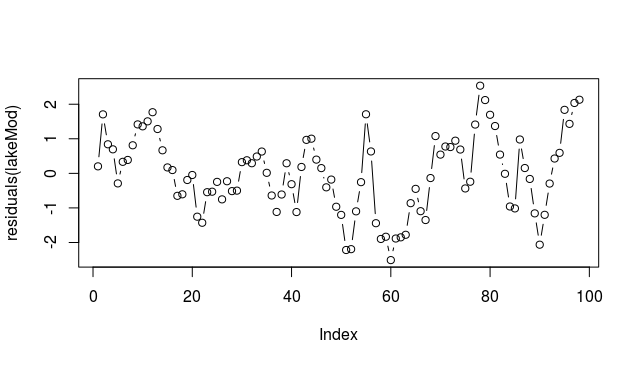
\includegraphics[width=60mm]{/home/taylor/UVa/all_teaching/4170_slides/1/1.4/pics/Rplot04}\\
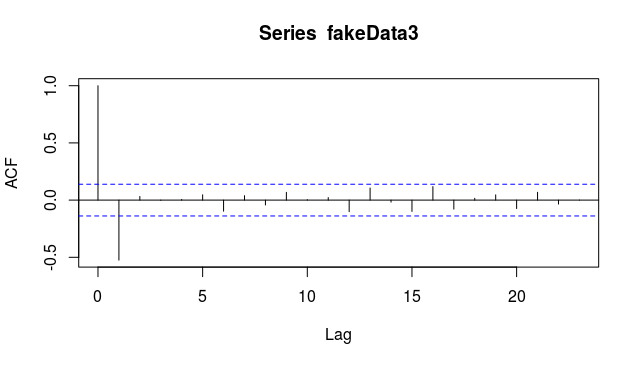
\includegraphics[width=60mm]{/home/taylor/UVa/all_teaching/4170_slides/1/1.4/pics/Rplot05}
\end{center}


\end{frame}

%----------------------------------------------------------------------------------------

\begin{frame}[fragile]
\frametitle{Test Yourself 3}

Answer: MA(1) with Gaussian Noise
\begin{verbatim}
fakeData3 <- arima.sim(list(ma=c(-.9)), n = 200)
plot(fakeData3, type = "b")
acf(fakeData3)
\end{verbatim}

\end{frame}


\end{document} 